%======================================================================
%  UPES  |  School of Computer Science  |  Mid-Sem Assignment Report
%  Template for Applied Machine Learning (CSAI2017P) and
%  Design and Analysis of Algorithms (CSEG3053)
%
%  HOW TO USE
%  1. Overleaf -> New Project -> Upload Project -> choose this .zip.
%     (Or: New Project -> Blank, paste this file, and upload references.bib.)
%  2. Fill in the details in the "YOUR DETAILS" block below.
%  3. Replace every section's placeholder text with your own writing.
%  4. The blue "Guidance" boxes tell you what each section needs.
%     When you are finished, change \showguidancetrue to
%     \showguidancefalse and they will disappear from the PDF.
%======================================================================
\documentclass[11pt,a4paper]{article}

%---------------- Packages ----------------
\usepackage[margin=2.3cm]{geometry}
\usepackage[T1]{fontenc}
\usepackage{amsmath,amssymb}
\usepackage{graphicx}
\usepackage{subcaption}
\usepackage{booktabs}
\usepackage{xcolor}
\usepackage{tikz}
\usetikzlibrary{arrows.meta,positioning,shapes.geometric}
\usepackage{pgfplots}
\pgfplotsset{compat=1.18}
\usepackage[ruled,vlined,linesnumbered]{algorithm2e}
\usepackage{listings}
\usepackage[most]{tcolorbox}
\usepackage{qrcode}
\usepackage{fancyhdr}
\usepackage[hidelinks]{hyperref}

\definecolor{upesnavy}{HTML}{1F3864}
\definecolor{guide}{HTML}{EAF1FB}
\definecolor{codebg}{HTML}{F7F7F7}

%================ YOUR DETAILS (edit these) ================
\newcommand{\studentname}{Anoushka Chawla}
\newcommand{\sapid}{590022992}
\newcommand{\batch}{B18}                          % B15, B16, B17, B18, B21 or B22
% \newcommand{\course}{Applied Machine Learning (CSAI2017P)}
\newcommand{\course}{Design and Analysis of Algorithms (CSEG3053)}
\newcommand{\topic}{Binary Search (Divide and Conquer)}
\newcommand{\animationlink}{https://github.com/your-username/binary-search-c}
\newcommand{\submissiondate}{\today}
%============================================================

\newif\ifshowguidance
\showguidancefalse   % guidance boxes hidden (set to \showguidancetrue to see them)

\newtcolorbox{guidancebox}{colback=guide,colframe=upesnavy!60,
  fonttitle=\bfseries\small,title=Guidance (delete or hide before submitting),
  fontupper=\small,boxrule=0.5pt,arc=2pt}
% Shows your screenshot if the file exists, otherwise a grey placeholder box,
% so the template compiles even before you add images.
\newcommand{\frameimg}[1]{\IfFileExists{#1}{\includegraphics[width=\linewidth]{#1}}%
  {\fbox{\parbox[c][0.7\linewidth][c]{0.92\linewidth}{\centering\small\color{gray}add\\\texttt{#1}}}}}
\newcommand{\guidance}[1]{\ifshowguidance\begin{guidancebox}#1\end{guidancebox}\fi}

\newtcolorbox{keyidea}{colback=upesnavy!4,colframe=upesnavy,
  fonttitle=\bfseries,title=Key Idea,boxrule=0.6pt,arc=2pt}

\lstset{basicstyle=\ttfamily\small,backgroundcolor=\color{codebg},
  frame=single,rulecolor=\color{gray!40},breaklines=true,
  numbers=left,numberstyle=\tiny\color{gray},keywordstyle=\color{upesnavy}\bfseries,
  commentstyle=\color{gray}\itshape,showstringspaces=false}

\pagestyle{fancy}\fancyhf{}
\lhead{\small\textcolor{upesnavy}{\topic}}
\rhead{\small\studentname\ (\sapid)}
\cfoot{\small\thepage}
\setlength{\headheight}{14pt}

\begin{document}

%======================== TITLE PAGE ========================
\begin{titlepage}
\centering
{\large\textsc{UPES, Dehradun}\par}
{\normalsize School of Computer Science $\cdot$ Artificial Intelligence Cluster\par}
\vspace{2.2cm}
{\color{upesnavy}\rule{\linewidth}{1.2pt}\par}
\vspace{0.6cm}
{\Huge\bfseries\color{upesnavy}\topic\par}
\vspace{0.4cm}
{\Large Mid-Semester Assignment Report\par}
\vspace{0.6cm}
{\color{upesnavy}\rule{\linewidth}{1.2pt}\par}
\vspace{2cm}
\begin{tabular}{rl}
\textbf{Course:}          & \course \\[3pt]
\textbf{Student:}         & \studentname \\[3pt]
\textbf{SAP ID:}          & \sapid \\[3pt]
\textbf{Batch:}           & \batch \\[3pt]
\textbf{Semester:}        & III (Aug--Dec 2026) \\[3pt]
\textbf{Submitted to:}    & Kunwar Siddharth, Assistant Professor \\[3pt]
\textbf{Date:}            & \submissiondate \\
\end{tabular}
\vfill
\begin{tabular}{c}
\qrcode[height=2.4cm]{\animationlink}\\[4pt]
\small Scan to open the animation / code
\end{tabular}
\end{titlepage}


%======================== ABSTRACT ========================
\begin{abstract}
In this report I look at binary search, a divide-and-conquer method for finding a
value in a sorted array. Instead of checking every element, it compares the key
with the middle element and throws away the half that cannot contain it. Because
the range halves every time, at most $\lfloor\log_2 n\rfloor+1$ comparisons are
needed, which is only about 20 for a million elements. I explain the idea in plain
words, work out the recurrence $T(n)=T(n/2)+\Theta(1)$, trace an example by hand,
and discuss time and space complexity and why the algorithm is correct. For the
demonstration I made an animated explainer video in Python and a C program with an
iterative and a recursive version. The C program prints every \texttt{lo}, \texttt{mid} and \texttt{hi} step, runs ten test cases,
and counts comparisons against linear search. The one thing to take away is that
every comparison removes half of what is left.
\end{abstract}

\tableofcontents
\newpage

%======================== 1 INTRODUCTION ========================
\section{Introduction}
\guidance{State the problem, where it sits in the course, and one real-world example.}

Searching means this: we have $n$ items and a target value (the key), and we want
to know where the key is, or that it is not there at all. When the items are in no
particular order we may have to look at every one of them, which takes $\Theta(n)$
time. When they are sorted we can do much better, and binary search is the
standard way to find the key in $O(\log n)$ time~\cite{cormen2022,knuth1998}.

A simple example is finding a word in a printed dictionary. Nobody starts at page
one. You open it somewhere near the middle, see whether your word comes before or
after that page, and repeat in the right half. Databases, file systems and
library functions use the same idea. What surprised me while reading is how easy
it is to get wrong: Knuth mentions that the first binary search was published in
1946 but a fully correct version only appeared in 1962~\cite{knuth1998}, and
Bentley reports that many professional programmers made mistakes when asked to
write it~\cite{bentley2000}.

%======================== 2 INTUITION ========================
\section{Intuition and Core Idea}
\guidance{Plain-words explanation with a diagram.}

Think of the guessing game where I pick a number between 1 and 100 and you may only
ask ``is it higher or lower than 50?''. Every answer cuts the possibilities in
half, so seven questions are always enough. Binary search is the same game played
on a sorted array, where the ``higher or lower'' answer comes from comparing
$a[\mathit{mid}]$ with the key.

\begin{keyidea}
Because the array is sorted, one comparison with the middle element tells us
which half the key must be in, so we can ignore the other half. If we keep doing
this the problem size goes $n,\ n/2,\ n/4,\dots$ until we find the key or run out
of elements.
\end{keyidea}

\begin{figure}[h]
\centering
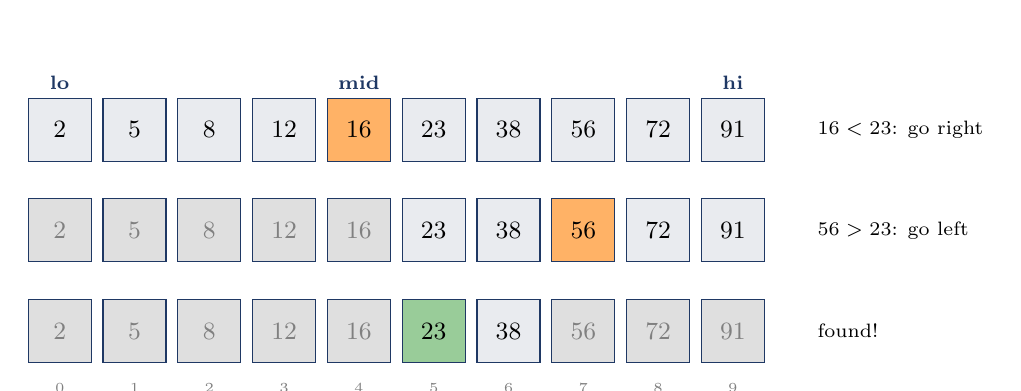
\begin{tikzpicture}[x=9.5mm,y=-8mm,
  cell/.style={draw=upesnavy,minimum size=8mm,inner sep=0pt,font=\small},
  act/.style={cell,fill=upesnavy!10},
  dead/.style={cell,fill=gray!25,text=gray},
  mid/.style={cell,fill=orange!60},
  hit/.style={cell,fill=green!50!black!40},
  lab/.style={font=\scriptsize\bfseries,text=upesnavy}]
\def\vals{2,5,8,12,16,23,38,56,72,91}
% row 0: initial
\foreach \v [count=\i from 0] in \vals {\node[act] at (\i,0) {\v};}
\node[lab] at (0,-0.75) {lo}; \node[lab] at (9,-0.75) {hi}; \node[lab] at (4,-0.75) {mid};
\node[mid] at (4,0) {16};
\node[anchor=west,font=\scriptsize] at (10.0,0) {$16<23$: go right};
% row 1
\foreach \v [count=\i from 0] in \vals {
  \ifnum\i<5 \node[dead] at (\i,1.6) {\v};\else\node[act] at (\i,1.6) {\v};\fi}
\node[mid] at (7,1.6) {56};
\node[anchor=west,font=\scriptsize] at (10.0,1.6) {$56>23$: go left};
% row 2
\foreach \v [count=\i from 0] in \vals {
  \ifnum\i<5 \node[dead] at (\i,3.2) {\v};\else
  \ifnum\i>6 \node[dead] at (\i,3.2) {\v};\else\node[act] at (\i,3.2) {\v};\fi\fi}
\node[hit] at (5,3.2) {23};
\node[anchor=west,font=\scriptsize] at (10.0,3.2) {found!};
\foreach \i in {0,...,9}{\node[font=\tiny,text=gray] at (\i,4.1) {\i};}
\end{tikzpicture}
\caption{Searching for $23$. Grey cells are already discarded, orange is the middle
element being compared, and green is the match. Ten elements needed only three
comparisons.}
\label{fig:idea}
\end{figure}

%======================== 3 MATHEMATICS ========================
\section{Mathematical Formulation}
\guidance{Define symbols, number equations, give recurrence and bound.}

Let $a[0..n-1]$ be sorted in non-decreasing order and let $k$ be the key. I keep a
\emph{search range} $[\mathit{lo},\mathit{hi}]$ which starts as $[0,n-1]$. The
middle index is
\begin{equation}
\mathit{mid} = \mathit{lo} + \left\lfloor \frac{\mathit{hi}-\mathit{lo}}{2} \right\rfloor .
\label{eq:mid}
\end{equation}
I write it like this instead of $\lfloor(\mathit{lo}+\mathit{hi})/2\rfloor$ because
$\mathit{lo}+\mathit{hi}$ can overflow for very large arrays, a bug that went
unnoticed in widely used library code for years~\cite{bloch2006}. After the
comparison, the range is updated like this:
\begin{equation}
\text{range}' =
\begin{cases}
\text{return } \mathit{mid} & a[\mathit{mid}] = k,\\
[\mathit{mid}+1,\ \mathit{hi}] & a[\mathit{mid}] < k,\\
[\mathit{lo},\ \mathit{mid}-1] & a[\mathit{mid}] > k.
\end{cases}
\label{eq:update}
\end{equation}
The search stops with ``not found'' when $\mathit{lo}>\mathit{hi}$.

\textbf{Recurrence.} Each step does one comparison and then continues on at most
half of the elements, so
\begin{equation}
T(n) = T\!\left(\tfrac{n}{2}\right) + \Theta(1),\qquad T(1)=\Theta(1).
\label{eq:rec}
\end{equation}
In the Master Theorem form $T(n)=aT(n/b)+\Theta(n^d)$ we have $a=1$, $b=2$ and
$d=0$, so $a=b^d$ and $T(n)=\Theta(n^d\log n)=\Theta(\log n)$. Unrolling gives the
same answer: after $j$ steps at most $n/2^j$ elements are left, and the range is
empty once $n/2^j<1$, that is, when $j>\log_2 n$. So the maximum number of
comparisons is
\begin{equation}
C_{\max}(n) = \lfloor \log_2 n \rfloor + 1 .
\label{eq:cmax}
\end{equation}

\begin{figure}[h]
\centering
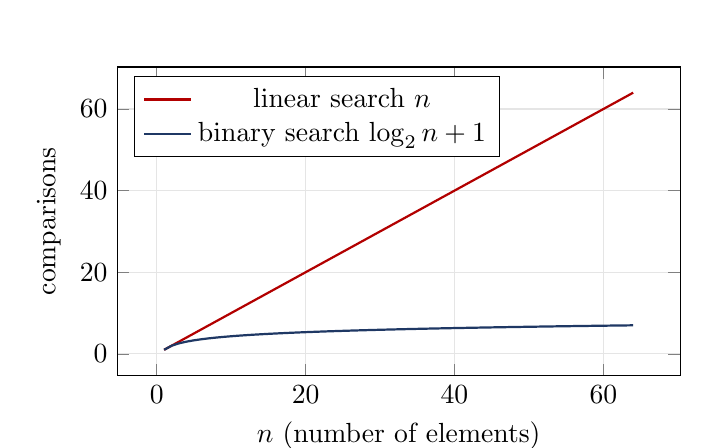
\begin{tikzpicture}
\begin{axis}[width=0.72\linewidth,height=5.5cm,
  xlabel={$n$ (number of elements)},ylabel={comparisons},legend pos=north west,
  grid=major,grid style={gray!20},domain=1:64,samples=64]
\addplot[red!70!black,thick]{x};         \addlegendentry{linear search $n$}
\addplot[upesnavy,thick]{ln(x)/ln(2)+1}; \addlegendentry{binary search $\log_2 n+1$}
\end{axis}
\end{tikzpicture}
\caption{Worst-case number of comparisons as $n$ grows. Compared with linear
search, the binary search curve is almost flat.}
\label{fig:plot}
\end{figure}

%======================== 4 ALGORITHM ========================
\section{Algorithm / Procedure}
\guidance{Pseudocode, then a short implementation excerpt.}

\begin{algorithm}[h]
\caption{Binary Search (iterative)}
\KwIn{sorted array $a[0..n-1]$, key $k$}
\KwOut{index of $k$ in $a$, or $-1$ if $k$ is absent}
$\mathit{lo}\leftarrow 0$;\quad $\mathit{hi}\leftarrow n-1$\;
\While{$\mathit{lo}\le \mathit{hi}$}{
  $\mathit{mid}\leftarrow \mathit{lo}+\lfloor(\mathit{hi}-\mathit{lo})/2\rfloor$\;
  \uIf{$a[\mathit{mid}]=k$}{\Return $\mathit{mid}$\;}
  \uElseIf{$a[\mathit{mid}]<k$}{$\mathit{lo}\leftarrow \mathit{mid}+1$\;}
  \Else{$\mathit{hi}\leftarrow \mathit{mid}-1$\;}
}
\Return $-1$\;
\end{algorithm}

In divide-and-conquer terms, the \emph{divide} step picks $\mathit{mid}$, the
\emph{conquer} step searches only the half that can contain $k$, and there is no
\emph{combine} step because the answer from that half is already the answer for
the whole array. The recursive version in my program follows this directly. Here
is the core of the C code (the full program is in \texttt{binary\_search.c}):

\begin{lstlisting}[language=C]
int binary_search_iter(const int a[], int n, int key)
{
    int lo = 0, hi = n - 1;
    while (lo <= hi) {
        int mid = lo + (hi - lo) / 2;   /* no overflow */
        if (a[mid] == key)     return mid;
        else if (a[mid] < key) lo = mid + 1;
        else                   hi = mid - 1;
    }
    return -1;                          /* not found */
}

int binary_search_rec(const int a[], int lo, int hi, int key)
{
    if (lo > hi) return -1;             /* base case */
    int mid = lo + (hi - lo) / 2;       /* divide    */
    if (a[mid] == key) return mid;
    if (a[mid] < key)                   /* conquer   */
        return binary_search_rec(a, mid + 1, hi, key);
    return binary_search_rec(a, lo, mid - 1, key);
}
\end{lstlisting}

%======================== 5 WORKED EXAMPLE ========================
\section{Worked Example (Step by Step)}
\guidance{Complete hand trace.}

I took the sorted array $a=[2,5,8,12,16,23,38,56,72,91]$ ($n=10$) and searched for
the key $k=23$.

\begin{table}[h]
\centering
\begin{tabular}{@{}cccccl@{}}
\toprule
\textbf{Step} & \textbf{lo} & \textbf{hi} & \textbf{mid} & $\mathbf{a[mid]}$ & \textbf{What happened} \\
\midrule
1 & 0 & 9 & 4 & 16 & $16<23$, discard left half, $\mathit{lo}=5$ \\
2 & 5 & 9 & 7 & 56 & $56>23$, discard right half, $\mathit{hi}=6$ \\
3 & 5 & 6 & 5 & 23 & $23=23$, \textbf{found at index 5} \\
\bottomrule
\end{tabular}
\caption{Trace of a successful search for $k=23$.}
\end{table}

It took 3 comparisons, while linear search would have needed 6. For an
\emph{unsuccessful} search I tried $k=40$. Steps~1 and~2 are the same as above
and the range becomes $[5,6]$. In step~3, $\mathit{mid}=5$ and $a[5]=23<40$, so
$\mathit{lo}=6$. In step~4, $\mathit{mid}=6$ and $a[6]=38<40$, so
$\mathit{lo}=7$. Now $\mathit{lo}=7$ is greater than $\mathit{hi}=6$, the range is
empty and the answer is $-1$ after 4 comparisons. This matches
$\lfloor\log_2 10\rfloor+1=4$ from Equation~\eqref{eq:cmax}.

%======================== 6 ANIMATION ========================
\section{Animation / Software Demonstration}
\guidance{Compulsory: tool, link, how to run, 3--4 key frames.}

\textbf{Tool used:} Python (matplotlib and ffmpeg) for the animated explainer video
(\texttt{make\_video.py} $\rightarrow$ \texttt{binary\_search\_explainer.mp4}, about
89 seconds), and a C program (\texttt{binary\_search.c}) that prints the same search
step by step in the terminal.\\
\textbf{Link:} \url{\animationlink}\\
\textbf{What the viewer sees:} the video starts with a guessing game (a number from
1 to 100) to show why halving works. It then searches the array
$[2,5,8,12,16,23,38,56,72,91]$ for 23 (found) and for 40 (not found). At each step
it shows \texttt{lo}, \texttt{hi} and \texttt{mid}, the formula for \texttt{mid},
the comparison, and the discarded half turning grey, with a running count of
comparisons. The last scenes show the recurrence $T(n)=T(n/2)+\Theta(1)$, a table
of comparisons for $n=10$ up to $10^6$, and three key takeaways. The C program
prints a row of indices, a row of values and a marker row, where \texttt{L},
\texttt{M} and \texttt{H} mark \texttt{lo}, \texttt{mid} and \texttt{hi}, a dot is an
element still in the range and \texttt{x} is one that has been discarded. It also
runs 10 self-tests and the same benchmark.\\
\textbf{What the viewer can change:} in the C program, the key and optionally their
own sorted array, from the command line. In \texttt{make\_video.py}, the array, keys
and timings can be edited in the script.\\
\textbf{How to run:} the C program (key first, then an optional sorted array) and the
video script:
\begin{lstlisting}[numbers=none,basicstyle=\ttfamily\footnotesize]
gcc -Wall -Wextra -O2 -o binary_search binary_search.c -lm
./binary_search                    # default demo, key 23
./binary_search 56                 # your own key
./binary_search 7 1 3 5 7 9        # key 7 in your own sorted array

pip install matplotlib             # ffmpeg must also be installed
python make_video.py render        # creates binary_search_explainer.mp4
\end{lstlisting}

Part of the actual program output for the default run:
\begin{lstlisting}[numbers=none,basicstyle=\ttfamily\footnotesize]
Step 2: lo=5  hi=9  mid=7  a[mid]=56
  index :    0   1   2   3   4   5   6   7   8   9
  value :    2   5   8  12  16  23  38  56  72  91
  range :    x   x   x   x   x   L   .   M   .   H
  -> 56 > 23 : discard right half, hi = mid-1 = 6
\end{lstlisting}

\begin{figure}[h]
\centering
\begin{subfigure}{0.48\linewidth}\frameimg{figures/frame1.png}\caption{Start: $\mathit{lo}=0$, $\mathit{hi}=9$}\end{subfigure}\hfill
\begin{subfigure}{0.48\linewidth}\frameimg{figures/frame2.png}\caption{Step 1: $16<23$, go right}\end{subfigure}\\[6pt]
\begin{subfigure}{0.48\linewidth}\frameimg{figures/frame3.png}\caption{Step 2: $56>23$, go left}\end{subfigure}\hfill
\begin{subfigure}{0.48\linewidth}\frameimg{figures/frame4.png}\caption{Step 3: found at index 5}\end{subfigure}
\caption{Screenshots from the explainer video for the search for $23$. Grey cells have
been discarded, orange is \texttt{mid} and green is the match.}
\label{fig:frames}
\end{figure}

%======================== 7 ANALYSIS ========================
\section{Analysis}
\guidance{Complexities, correctness, comparison table.}

\subsection*{Time Complexity}
\textbf{Best case} $O(1)$: the key happens to be the first middle element.
\textbf{Worst and average case} $\Theta(\log n)$: every iteration halves the range,
so there are at most $\lfloor\log_2 n\rfloor+1$ iterations
(Equation~\eqref{eq:cmax}) and each one does a constant amount of work. My
benchmark agrees with this: for $n=10^6$ an absent key took exactly 20
comparisons, against $10^6$ for linear search.

\subsection*{Space Complexity}
The iterative version only stores \texttt{lo}, \texttt{hi} and \texttt{mid}, so it
uses $O(1)$ extra space. The recursive version adds one stack frame for every
halving, so it needs $O(\log n)$ space in the worst case. Neither one copies the
array.

\subsection*{Why the Method Works}
I used a loop invariant: \emph{if $k$ is in the array, then it is in
$a[\mathit{lo}..\mathit{hi}]$}. At the start the range is the whole array, so this
is true. If $a[\mathit{mid}]<k$, then because the array is sorted everything up
to $\mathit{mid}$ is $\le a[\mathit{mid}]<k$, so none of it can equal $k$ and
moving $\mathit{lo}$ to $\mathit{mid}+1$ loses nothing. The case
$a[\mathit{mid}]>k$ is symmetric. The range gets smaller in every iteration, so
the loop must stop, and if it stops with an empty range the invariant tells us
that $k$ is not in the array.

\textbf{Limitations.} The array has to be sorted, and sorting costs
$O(n\log n)$, so it is only worth it if we search many times. It also needs
random access, so it does not suit linked lists.

\begin{table}[h]
\centering
\begin{tabular}{@{}lll@{}}
\toprule
\textbf{Criterion} & \textbf{Binary search} & \textbf{Linear search} \\
\midrule
Main goal & find key by halving a sorted range & scan every element in turn \\
Time (worst) & $\Theta(\log n)$ & $\Theta(n)$ \\
Extra space & $O(1)$ iterative, $O(\log n)$ recursive & $O(1)$ \\
Strength & very fast on large data & works on unsorted data and linked lists \\
Limitation & needs sorted data with random access & slow for large $n$ \\
\bottomrule
\end{tabular}
\caption{Comparison with linear search.}
\end{table}

%======================== 8 APPLICATIONS ========================
\section{Applications}
\begin{enumerate}
\item \textbf{Database and file indexes:} sorted indexes let a lookup skip most of
the records, so finding one row among millions takes only about twenty
comparisons.
\item \textbf{Standard libraries:} C has a library function \texttt{bsearch} for
sorted arrays, and Kernighan and Ritchie also present a binary search
function~\cite{kr1988}. Other languages have similar functions.
\item \textbf{Finding a bug or a threshold:} \texttt{git bisect} halves the range
of commits to find the one that introduced a bug, and the bisection method for
finding roots of an equation works the same way.
\end{enumerate}

%======================== 9 CONCLUSION ========================
\section{Conclusion}
Binary search turns a sorted array into a problem that halves itself at every
step, which gives $\Theta(\log n)$ time and $O(1)$ extra space for the iterative
version. Writing the C trace made \texttt{lo}, \texttt{mid} and \texttt{hi} much
clearer to me, and it showed how easy it is to slip on the boundaries
(\texttt{mid+1}, \texttt{mid-1}, \texttt{lo<=hi}) or on the midpoint formula. One
thing I would like to explore next is how interpolation search and exponential
search behave when the data is not evenly spread out.

%======================== DECLARATION ========================
\section*{Declaration of AI Tool Use}
\addcontentsline{toc}{section}{Declaration of AI Tool Use}
\noindent\textbf{Tools used:} Claude (Anthropic)\\
\textbf{What for:} drafting the report and code, corrections and reviewing\\
\textbf{Approximate share of AI-generated content:} \dots\%\\[6pt]
I confirm that this report and the animation are my own individual work.\\[14pt]
Signature: \rule{4cm}{0.4pt} \hfill Date: \rule{3cm}{0.4pt}

%======================== REFERENCES ========================
\bibliographystyle{ieeetr}
\bibliography{references}

\end{document}
